\documentclass{tufte-handout}

\title{CIS 2033 Lecture 1, Spring 2017\thanks{Readings from the textbook: \\Chapter 1, Sec 1}}

\author[David Dobor]{Instructor: David Dobor}

\date{January 2017} % without \date command, current date is supplied

%\geometry{showframe} % display margins for debugging page layout

\usepackage{graphicx} % allow embedded images
  \setkeys{Gin}{width=\linewidth,totalheight=\textheight,keepaspectratio}
  \graphicspath{{graphics/}} % set of paths to search for images
\usepackage{amsmath}  % extended mathematics
\usepackage{booktabs} % book-quality tables
\usepackage{units}    % non-stacked fractions and better unit spacing
\usepackage{multicol} % multiple column layout facilities
\usepackage{lipsum}   % filler text
\usepackage{fancyvrb} % extended verbatim environments
  \fvset{fontsize=\normalsize}% default font size for fancy-verbatim environments

% Standardize command font styles and environments
\newcommand{\doccmd}[1]{\texttt{\textbackslash#1}}% command name -- adds backslash automatically
\newcommand{\docopt}[1]{\ensuremath{\langle}\textrm{\textit{#1}}\ensuremath{\rangle}}% optional command argument
\newcommand{\docarg}[1]{\textrm{\textit{#1}}}% (required) command argument
\newcommand{\docenv}[1]{\textsf{#1}}% environment name
\newcommand{\docpkg}[1]{\texttt{#1}}% package name
\newcommand{\doccls}[1]{\texttt{#1}}% document class name
\newcommand{\docclsopt}[1]{\texttt{#1}}% document class option name
\newenvironment{docspec}{\begin{quote}\noindent}{\end{quote}}% command specification environment

\begin{document}

\maketitle% this prints the handout title, author, and date

\begin{abstract}
\noindent
We discuss administrativia and dive right into the material.
\end{abstract}

%\printclassoptions

\section{Introduction}\label{sec:intro}
A probabilistic model is \marginnote{A Probabilistic Model}a quantitative description of 
a phenomenon or an experiment
whose outcome is uncertain. Putting together such a model involves two key steps. First, we need to
describe the possible outcomes of the experiment. This is done by specifying a so-called sample space.
And then by specifying a probability law, which assigns probabilities to outcomes or to collections of
outcomes.

The probability law tells us, for example, whether one outcome is much more likely than some other
outcome. Probabilities have to satisfy certain basic properties in order to be meaningful.  For example,
probabilities cannot be negative. These are the axioms of probability theory.

Interestingly, there will be very few axioms, but they are
powerful, and we will see that they imply many other
properties that were not part of the axioms.

We will then go through a couple of very simple examples involving models with either discrete or
continuous outcomes. As you will see many times in this class, discrete models are conceptually
much easier. Continuous models involve some more sophisticated concepts, and we will point out some
of the subtle issues that arise. 

Finally, we will talk a little bit about the big picture, about the role of
probability theory, and its relation with the real world.

\section{Building the Probabilistic Model}\label{sec:model-building}

Putting together a probabilistic model-- that is, a model of a random phenomenon or a random
experiment-- involves two steps:

\begin{enumerate}
\item In the first step we describe the possible outcomes of the phenomenon or
experiment of interest.
\item In the second step we describe our beliefs about the likelihood of the different
possible outcomes by specifying a probability law.
\end{enumerate}


\subsection{Step1: Describing Outcomes}\label{sec:outcomes}

So let's start with the description of the possible outcomes of
an experiment. We carry out some experiment: for example, we flip a coin, or maybe we flip five coins
simultaneously, or maybe we roll a die. Whatever that experiment is, it has a number of possible
outcomes, and we start by making a list of the possible outcomes.


\begin{marginfigure}
  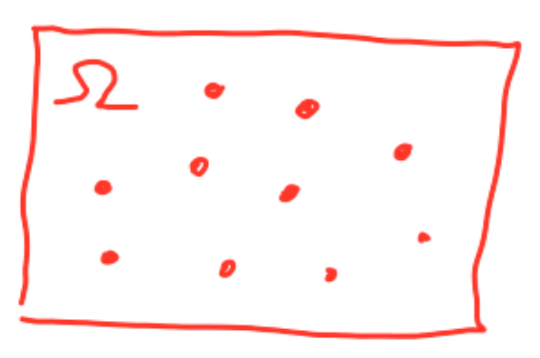
\includegraphics[width=\linewidth]{Omega}
  \caption{The sample space $\Omega$ can be represented by a  drawing like this one. Each individual dot represents an outcome. The outcomes are mutually exclusive and make up the entire space $\Omega$.}
  \label{fig:marginfig}
\end{marginfigure}

We create a set that we usually denote by capital omega: $\Omega$. That set is called the sample 
space and is the set of all possible outcomes of our experiment. 
The elements of that set should have certain properties. Namely, the elements \textit{should be 
mutually exclusive and collectively exhaustive.}

What does that mean? Mutually exclusive means that, if at 
the end of the experiment, I tell you that a particular 
outcome happened (a red dot),  then it should not be possible for another outcome (some other red dot) also to have happened. At the end of the
experiment, there can only be one of the outcomes that has happened.

Being collectively exhaustive means something else -- that, 
together, all of these elements of the set
exhaust all the possibilities. So no matter what, at the end, you will be able to point to one of the
outcomes and say, that's the one that occurred. 

To summarize-- this set should be such that, at the end
of the experiment, you should be always able to point to one, and exactly one, of the possible outcomes
and say that this is the outcome that occurred.

Physically different outcomes should be distinguished in the sample space and correspond to distinct
points. But when we say physically different outcomes, what do we mean? We really mean different in
all relevant aspects but perhaps not different in irrelevant aspects.

% let's start a new thought -- a new section
\newthought{Example 1.} Let's make more precise what I mean by that by looking at a very simple, and maybe silly, example,
which is the following. Suppose that you flip a coin and you see whether it resulted in heads or tails. So
you have a perfectly legitimate sample space for this experiment which consists of just two points -- one
head and one tail.
\begin{marginfigure}
  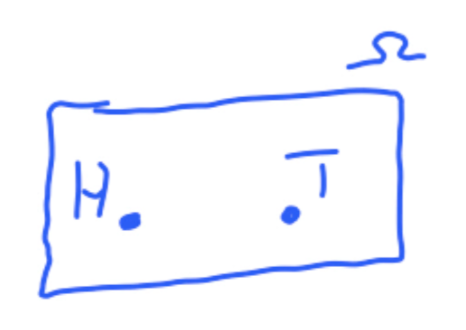
\includegraphics[width=\linewidth]{HeadsTails}
  \caption{A sample space $\Omega$ with two outcomes.}
  \label{fig:marginfig}
\end{marginfigure}

Together these two outcomes exhaust all possibilities. And the two outcomes are mutually exclusive. So
this is a legitimate sample space for this experiment. Now suppose that while you were flipping the
coin, you also looked outside the window to check the weather. And then you could say that my sample
space is really heads, and it's raining. Another possible outcome is heads and no rain. Another
possible outcome is tails, and it's raining, and, finally, another possible outcome is tails and no rain.
This set consisting of four elements (see Fig 3), is also a perfectly legitimate sample space for the experiment of
flipping a coin. The elements of this sample space are mutually exclusive and collectively exhaustive.
Exactly one of these outcomes will have materialized at the end of the
experiment.
\begin{marginfigure}
  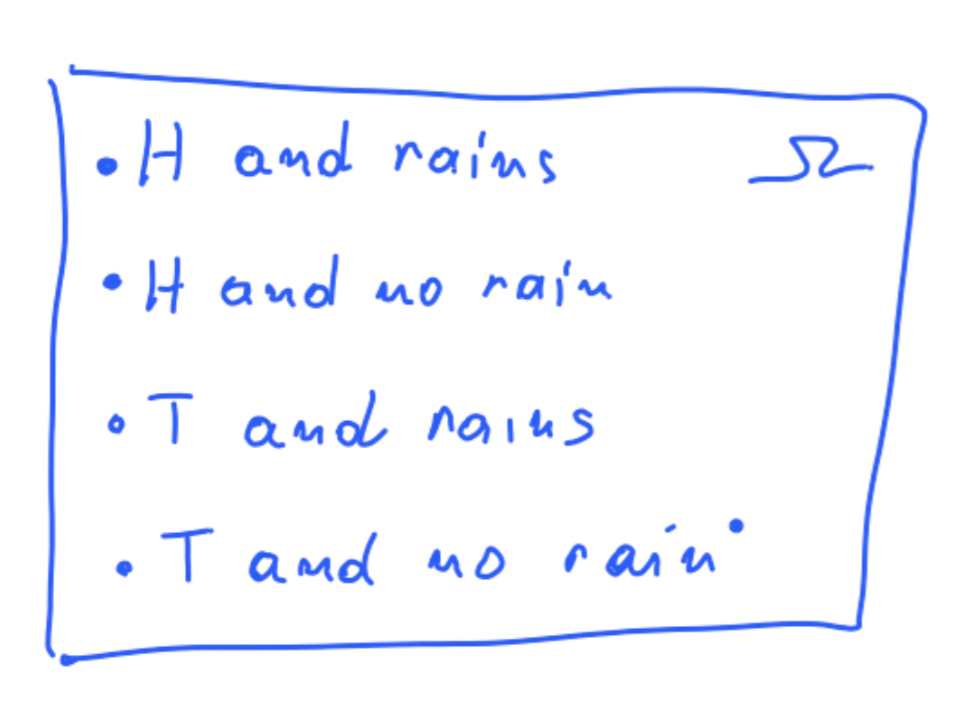
\includegraphics[width=\linewidth]{HeadsTailsRain}
  \caption{A sample space $\Omega$ with four outcomes.}
  \label{fig:marginfig}
\end{marginfigure}
So which sample space is the correct one? This sample space, the second one, involves some
irrelevant details. So the preferred sample space for describing the flipping of a coin is the 
simpler one, the first one, which is sort of at the right granularity, given what we're
interested in.

Ultimately, the question of which one is the right sample space depends on what kind of questions
you want to answer. For example, if you have a theory that the weather affects the behavior of coins,
then, in order to play with that theory, or maybe check it out, then you might
want to work with the second sample space.
This is a common feature in all of science. Whenever you put together a model, you need to decide
how detailed you want your model to be. And the right level of detail is the one that captures those
aspects that are relevant and of interest to you.

\newthought{\textit{Check Your Understanding: }} For the experiment of flipping a coin, and for each one of the following choices, determine whether we have a legitimate sample space:
\begin{align}
\Omega &= \{ \text{Heads and it is raining, Heads and it is not raining, Tails}\} \\
\Omega &= \{ \text{Heads and it is raining, Tails and it is not raining, Tails}\}
\end{align}

\vspace{0.5cm}

\newthought{Let us } now look at some more examples of sample spaces. Sample spaces are sets, and a set can be
discrete, finite, infinite, continuous, and so on.

\newthought{Example 2: } Let us start with a simpler case in which we have a
sample space that is discrete and finite.
The particular experiment we will be looking at is the following. We take a very special die, a tetrahedral
die. So it's a die that has four faces numbered from 1 up 4. We roll it once. And then we roll it again.
Were not dealing here with two probabilistic experiments. We're dealing with a single probabilistic
experiment that involves two rolls of the die within that experiment. What is the sample space of that
experiment? 

\begin{marginfigure}
  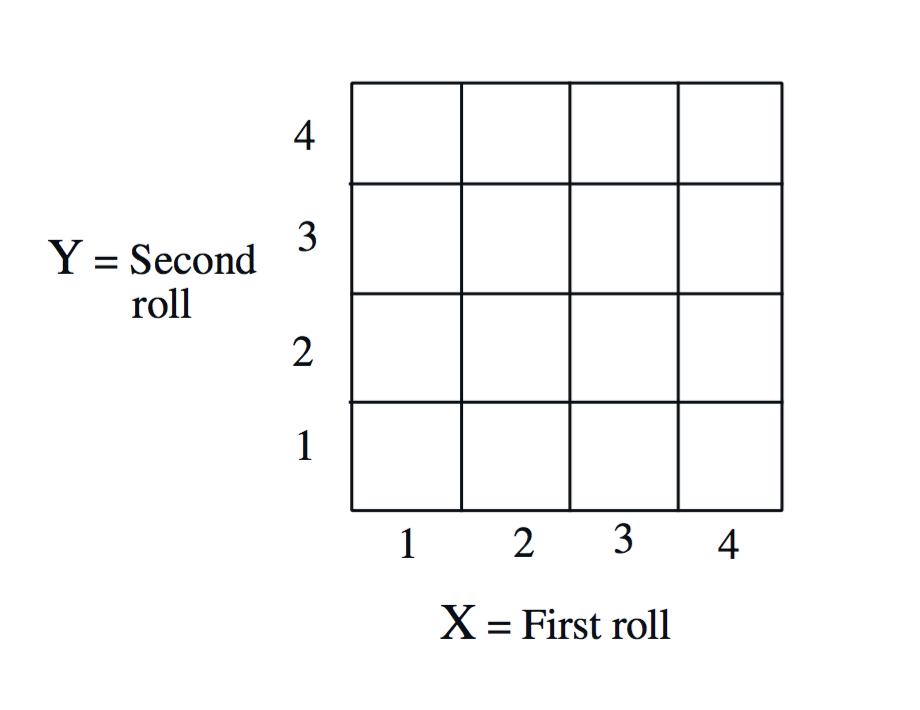
\includegraphics[width=\linewidth]{Dice2}
  \caption{A representation for two rolls of a 4-sided die.}
  \label{fig:marginfig}
\end{marginfigure}




Well, one possible representation is the following. We take note of the result of the first roll.
And then we take note of the result of the second roll. And this gives us a pair of numbers.
Each one of the possible pairs of numbers corresponds to one of the little squares in this diagram. For
example, if the first roll is 1 and the second is also 1, then this particular outcome can be represented 
by the lowest leftmost square. If the first roll is it 2 and the second is a 3, then this particular outcome 
can be represented by the square we might call "(2, 3)" (See Fig 5). If the first roll is a 3 and then
the next one is a 2, then this particular can be represented by the square we might call "(3, 2)", and so on.

Notice that the outcomes "(2, 3)"  and "(3, 2)" are pretty closely related. In both cases, we observe a 2 and we
observe a 3. But we distinguish those two outcomes because in those two outcomes, the 2 and the 3
happen in different order, and the order in which they appear may be a detail which is of interest to us. So we make this
distinction in the sample space and we keep the (3, 2) and the (2, 3) as separate outcomes.

\begin{marginfigure}
  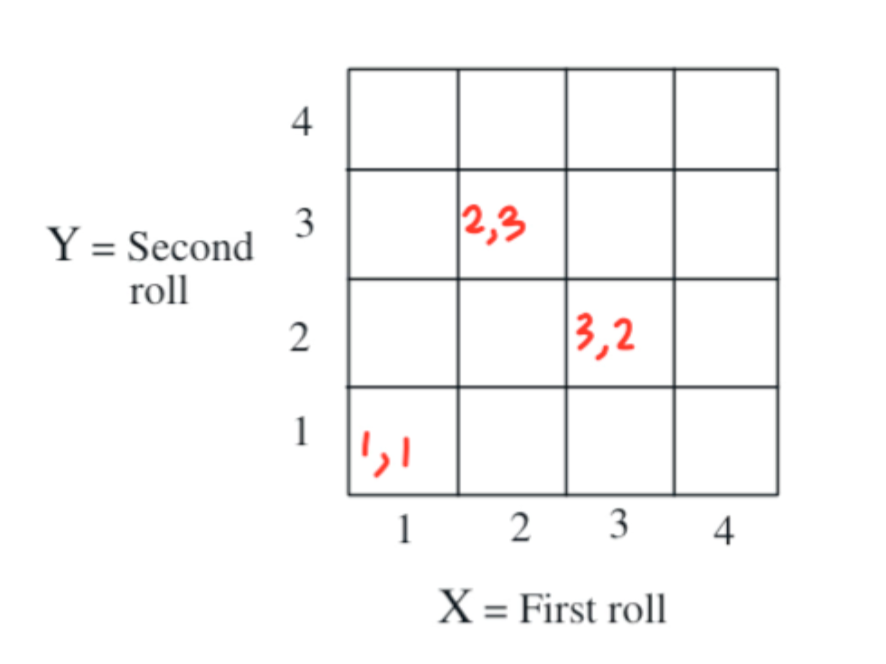
\includegraphics[width=\linewidth]{Dice2Annotated}
  \caption{We distinguish between outcomes (2, 3) and (3, 2).}
  \label{fig:marginfig}
\end{marginfigure}


\vspace{0.7cm}
Now, this is a case of a model in which the probabilistic experiment can be described in phases or
stages. We could think about rolling the die once and then going ahead with the second roll. So we
have two stages.

A very useful way of describing the sample space of experiments-- whenever we have an experiment
with several stages, either real stages or imagined stages. A very useful way of describing it is by
providing a sequential description in terms of a tree. We call a diagram of the kind shown in Figure 6 a 
tree. You can think of the leftmost point on this picture as the \textit{root} of the tree from which 
you start. The endpoints of the tree are usually called \textit{leaves}.

\begin{marginfigure}
  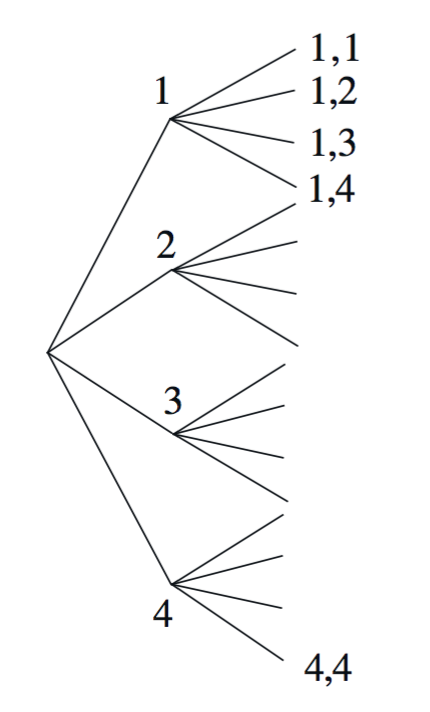
\includegraphics[width=\linewidth, height=5cm]{Dice2Sequential}
  \caption{A different representation for the same experiment.}
  \label{fig:marginfig}
\end{marginfigure}


So here's how we read this tree. The experiment starts. We carry out the first phase, which in this case is the first roll, and we see
what happens. So maybe we get a 2 in the first roll. If that's the case, we follow the branch from the root that leads to the "2". We then continue the experiment by rolling the die again, and we take note of what happened in the
second roll. Maybe the result was a 3 this time. We then follow that branch from "2" that reads "(2, 3)", and so on.

Notice that in this tree we once more have a distinction. The outcome 2 followed by a 3 is
different from the outcome 3 followed by a 2. In both cases, we have 16 possible outcomes. 4 times 4 makes 16. And similarly, if you count, the
number of leaves is equal to 16. 

\vspace{0.7cm}

The previous example involves a sample space that is \textit{discrete and
finite}: there are only 16 possible outcomes. But sample spaces can also be infinite; they can
also be continuous sets.

\newthought{Example 3: } Here's an example of an experiment that involves a continuous sample space. Here we have a
rectangular target which is the unit square. You throw a dart on that target. Suppose that you
are so skilled that no matter what, when you throw the dart, it always falls inside the target.

\begin{marginfigure}
  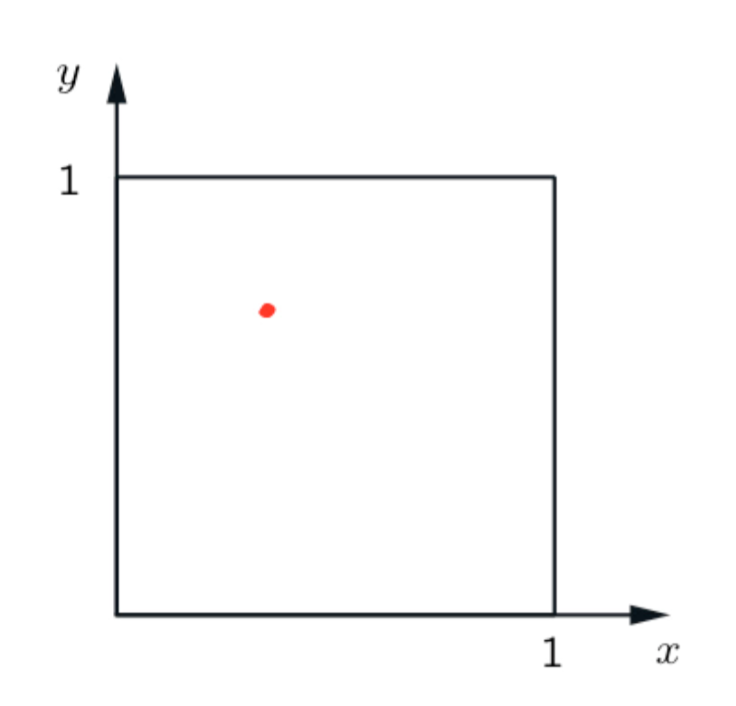
\includegraphics[width=\linewidth]{ContinousSpace}
  \caption{An example of a coninuous outcome space - throw darts into the square $(x, y)$ such that $0 \leq x, y \leq 1$.}
  \label{fig:marginfig}
\end{marginfigure}



Once the dart hits the target, you record the coordinates $x$ and $y$ of the particular point that resulted
from your throw. You record $x$ and $y$ with infinite precision. So $x$ and $y$ are real numbers. In
this experiment, the sample space is just the set of $x, y$ pairs that lie between 0 and 1.



\newthought{\textit{Check Your Understanding: }} Paul checks the weather forecast. If the forecast is good, Paul will go out for a walk. If the forecast is bad, then Paul will either stay home or go out. If he goes out, he might either remember or forget his umbrella. In the tree diagram below, identify the leaf that corresponds to the event that the forecast is bad and Paul stays home.

\begin{figure}
  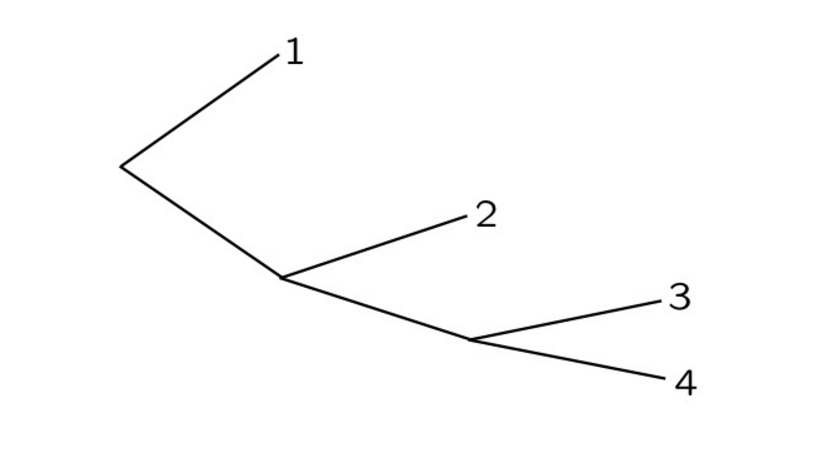
\includegraphics[height=5cm]{Question2}
\end{figure}

\vspace{0.5cm}



\subsection{Step 2: Describing Our Beliefs about the Outcomes}\label{sec:probability-space}

We now come to the second and much more interesting part. We need to specify which outcomes are
more likely to occur and which ones are less likely to occur, and we will do that by assigning
probabilities to the different outcomes.

However, as we try to do this assignment, we run into a difficulty, which is the following.
Remember the previous experiment involving a continuous sample space, which was the unit square
and in which we throw a dart at random and record the point that occurred?

In this experiment, what do you think is the probability of a particular point? Let's say what is the
probability that my dart hits exactly the center of this square. Well, this probability would be essentially
$0$. Hitting the center exactly with infinite precision should be $0$.

And so it's natural that in such a continuous model any individual point should have a $0$ probability. For
this reason instead of assigning probabilities to individual points, we will instead assign probabilities to
whole sets, that is, to subsets of the sample space.

\begin{marginfigure}
  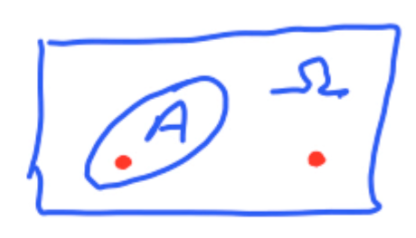
\includegraphics[width=\linewidth]{Subset}
  \caption{In the continuous case, we assign probabilities to whole whole sets, not to individual points.}
\end{marginfigure}


So here we have our sample space, which is some abstract set $\Omega$. Here is a subset of the sample
space. Call it $A$. We're going to assign a probability to that subset $A$, which we're going to denote
with $P(A)$, which we read as the probability of set $A$. So probabilities will be assigned to subsets.

\begin{marginfigure}
  
\includegraphics[width=1.5cm, height=1.5cm]{ProbA}
  \caption{Probability assigned to set $A$.}
\end{marginfigure}

And these will not cause us difficulties in the continuous case because even though individual points
would have $0$ probability, if you ask me what are the odds that my dart falls in the upper half, let's say,
of this diagram, then that should be a reasonable positive number. So even though individual outcomes
may have probabilities equal to zero, sets of outcomes in general would be expected to have positive probabilities.

\begin{marginfigure}
  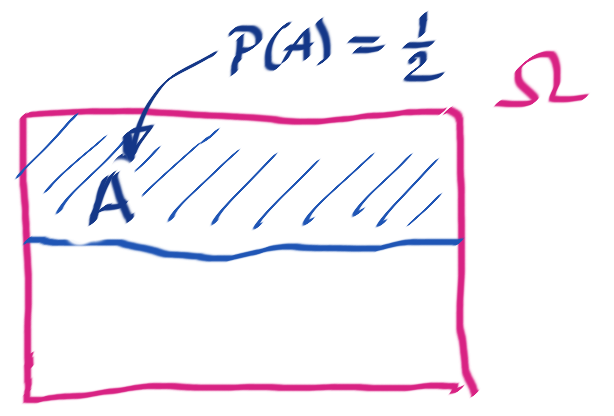
\includegraphics[width=\linewidth]{UpperHalf}
  \caption{This upper half of the samples space gets $P(A)$ of $\frac{1}{2}$ assigned to it.}
\end{marginfigure}


So, to repeat, we're going to assign probabilities to the various subsets of the sample space. And
here comes a piece of terminology: 

\vspace{0.5cm}
\emph{A subset of the sample space is called an event.}
\vspace{0.5cm}

Why is it called an event? Because once we carry out the experiment and we observe the outcome of the
experiment, either that outcome is inside the set $A$ -- and in that case we say that event $A$ has occurred -- or
the outcome falls outside the set $A$ \marginnote{A subset of the sample space is called an event.}in which case 
we say that event $A$ did not occur. 

\subsection{Axioms of Probability}\label{sec:probability-axioms}

Now we want to move on and describe certain rules - "rules of the game" in probabilistic models,
which are basically the rules that these probabilities should satisfy. They shouldn't be completely
arbitrary. First, by convention, probabilities are always given in the range between $0$ and $1$. Intuitively, $0$
probability means that we believe that something practically cannot happen. And probability of 1 means
that we're practically certain that an event of interest is going to happen.


These rules that any probabilistic model
should satisfy are called the axioms of probability theory. 

\newthought{Our first axiom} is a nonnegativity axiom.
Namely, probabilities will always be non-negative numbers. It's a reasonable rule. 
\begin{marginfigure}
  
\includegraphics[width=1.5cm, height=1cm]{Axiom1}
  \caption{Axiom 1: Nonnegativity.}
\end{marginfigure}

\newthought{The second rule} is
that if the subset that we're looking at is actually not a subset but is the entire sample space $\Omega$, the
probability of it should always be equal to 1.
\begin{marginfigure}
  
\includegraphics[width=1.5cm, height=1cm]{Axiom2}
  \caption{Axiom 2: Normalization.}
\end{marginfigure}

What does that mean? We know that the outcome is going to be an element of the sample space. This
is the definition of the sample space. So we have absolute certainty that our outcome is going to be in
$\Omega$. Or, using a different language, we have absolute certainty that event $\Omega$ is going to 
occur. And we capture this certainty by saying that $P(\Omega) = 1$.


These two axioms are pretty simple and very intuitive. The more interesting axiom is the next one that
says something a little more complicated. Before we discuss that particular axiom, a quick reminder
about set theoretic notation. If we have two sets, let's say a set $A$, and another set, another set $B$, we
use the notation $A \cap B$ to refer to the collection of elements
that belong to both $A$ and $B$. So in Figure 13, the \emph{intersection} of $A$ and $B$ is the shaded set. We use
the notation $A \cup B$ to refer to the set of elements that belong to $A$ or to $B$ or to
both. So in Figure 14, the union of the two sets would be the set represented by the blue shaded area.
\begin{marginfigure}
  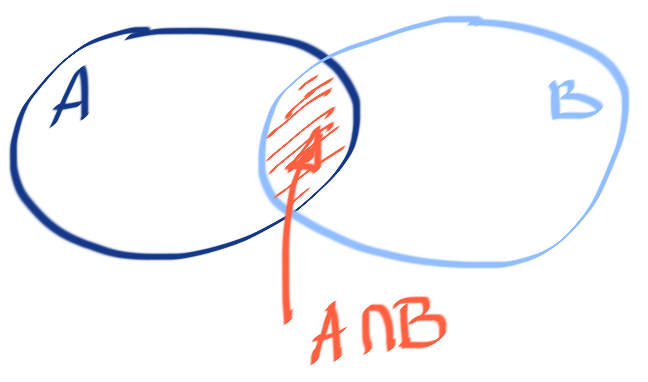
\includegraphics[width=\linewidth]{Intersection}
  \caption{Intersection of Events.}
\end{marginfigure}

\begin{marginfigure}
  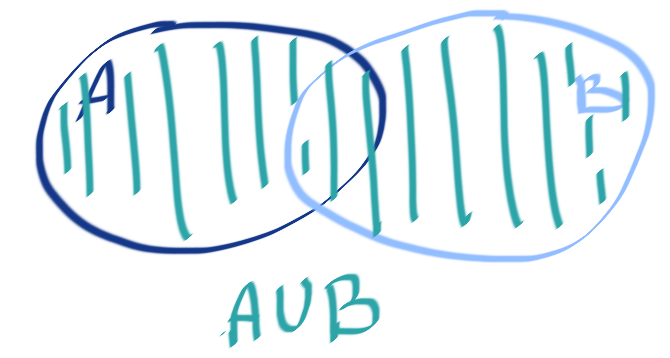
\includegraphics[width=\linewidth]{Union}
  \caption{Union of Events.}
\end{marginfigure}

\newthought{Now let us look at the third axiom.} It says that if we have two events, i.e. two subsets of the 
sample space, which are disjoint, then the probability that the outcome of the experiment falls
in the union of $A$ and $B$ is equal to the sum of
the probabilities of these two sets.
(As shown in Figure 15, two sets
being disjoint means that their intersection has no elements, i.e. their intersection is the empty set, and
we use this symbol $\emptyset$ to denote the empty set) \textit{This is called the additivity axiom.} It says that we can add
probabilities of different sets when those two sets are disjoint.

\begin{marginfigure}
  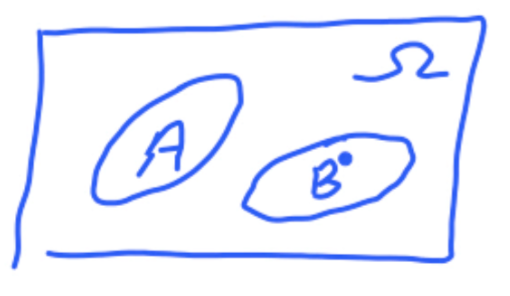
\includegraphics[width=\linewidth]{NonIntersecting}
  \caption{Non Intersecting of Events.}
\end{marginfigure}


\begin{marginfigure}[2cm]
  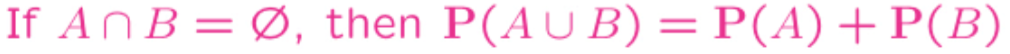
\includegraphics[width=\linewidth]{Axiom3}
  \caption{Axiom 3: Additivity.}
\end{marginfigure}

In some sense we can think of probability as being one pound of some substance (of course your are free to 
think of ice-cream here) which is spread over our sample space and $P(A)$ is how much of that substance 
is sitting on top of a set $A$. What this axiom is saying is that whenever the sets $A$ and $B$ are disjoint 
from each other, the total amount of that substance sitting on top of $A$ and $B$ is how much is sitting on 
top of $A$ plus how much is sitting on top of $B$. 

\newthought{And one final note:} The additivity axiom needs to be refined a bit. We will talk about that a little 
later. Other than this refinement, these three axioms are the only requirements in order to have a legitimate 
probability model. At this point you may ask, shouldn't there be more requirements? Shouldn't we, for example,
say that probabilities cannot be greater than 1? Yes and no. We do not want probabilities to be larger
than 1, but we do not need to say it. As we will see in the next segment, such a requirement follows
from what we have already said. And the same is true for several other natural properties of
probabilities.

\newthought{\textit{Check Your Understanding: }} Let $A$ and $B$ be events, with $P(A)=0.6$ and $P(B)=0.7$. Can these two events be disjoint?

\vspace{0.5cm}

\end{document}
